\documentclass[conference]{IEEEtran}
\IEEEoverridecommandlockouts
% The preceding line is only needed to identify funding in the first footnote. If that is unneeded, please comment it out.
\usepackage{cite}
\usepackage{amsmath,amssymb,amsfonts}
\usepackage{algorithmic}
\usepackage{graphicx}
\usepackage{textcomp}
\usepackage{xcolor}
\usepackage{stfloats}
\usepackage{minted}



\def\BibTeX{{\rm B\kern-.05em{\sc i\kern-.025em b}\kern-.08em
    T\kern-.1667em\lower.7ex\hbox{E}\kern-.125emX}}



\begin{document}

\title{emDB: Embedded databases as schema compilers %\\
    % {\footnotesize \textsuperscript{*}Note: Sub-titles are not captured in Xplore and
    % should not be used}
    % \thanks{Identify applicable funding agency here. If none, delete this.}
}

\author{
    \IEEEauthorblockN{Oliver Killane}
    \IEEEauthorblockA{\textit{Imperial College London} \\
        London, United Kingdom \\
        ok220@ic.ac.uk}
    \and
    \IEEEauthorblockN{Holger Pirk}
    \IEEEauthorblockA{\textit{Imperial College London} \\
        London, United Kingdom \\
        hlgr@ic.ac.uk}
    \and
    \IEEEauthorblockN{ChatGPT 4o}
    \IEEEauthorblockA{\textit{OpenAI} \\
        San Francisco, California}
}

\maketitle

\begin{abstract}
    In this paper, we introduce emDB - the easy macro database system embeddable in rust programs. 
    EmDB challenges traditional assumptions about embedded databases, such as the
    need for a SQL interface, schema changes, and ad-hoc queries. By using a static schema and known 
    parameterized queries, emDB moves query parsing, semantic analysis, and code generation to compile 
    time, and eliminates the need for a complex execution engine.

    Implemented as a Rust procedural macro, emDB reads schemas and queries, selects appropriate data
    structures, reports type and query errors and generates optimized query code at compile time. 
    This approach, based on a known set of queries, allows for the use of optimal data structures 
    and integrates seamlessly with standard debugging, benchmarking, verification, and testing tools. 
    EmDB also makes use of language-specific features like move semantics and borrow checking, providing 
    an efficient and safe interface for developers, including support for user-defined types and code to be embedded 
    into the database.
\end{abstract}

\begin{IEEEkeywords}
    databases, compilers, rust, macros
\end{IEEEkeywords}

\section{Introduction}

\begin{figure*}[b]
    \centering
    
\includegraphics[width=\textwidth]{_diagrams/problem_space.pdf}
    \caption{Embedded databases on a spectrum of abstraction}
    \label{fig:abstraction-spectrum}
\end{figure*}

Embedded data processing tools can be placed on a spectrum of abstraction.

At the lower end of the spectrum, manual implementation requires developers to implement operators,
design data structures, and conduct thorough testing. While this approach demands considerable effort,
it can yield optimal performance results due to the high level of control it offers.

At a higher abstraction, dataframes provide a set of pre-defined operators, simplifying the development
process. However, users still need to compose operators manually. Notably, there is no compilation
step in dataframe libraries that allows for an optimiser to determine data structure and operator implementation choices
based on the entire query and schema context.

LINQ (Language Integrated Query) offers a higher level of query abstraction, including a SQL-like
interface, yet users are still responsible for making data structure choices and selecting operator
implementations.

These methods generally impose several restrictions on the user:
\begin{itemize}
    \item The schema is static.
    \item All parameterized queries are known at application compile time.
\end{itemize}

Transitioning to a full SQL-like abstraction, which includes transactions, operator and data structure
selection, and query optimization, there is a discontinuity. This level of abstraction
removes the aforementioned restrictions at significant cost.

Moving query parsing, planning, optimization, as well as schema altering queries to application
runtime incurs significant implementation complexity (ratalogue management, runtime types information)
and runtime overhead (for example query compilation in codegen, or virtual calls in interpreted queries).

Additionally some level of serialization/deserialization is needed to move data from the host application
(i.e. statically typed, without a stable ABI) into the embedded database (i.e. dynamically typed, over SQL string interface and/or C-ABI).

Given for the vast majority of applications using embedded databases, the queries are known, and the schema does not change, we argue there 
is no clear rationale for this disjointness in the spectrum of abstraction, nor for the absence
of a higher level of abstraction that still benefits from the restrictions present in lower levels.

\section{Schema Compilation Advantage}

\begin{figure*}[b]
    \centering
    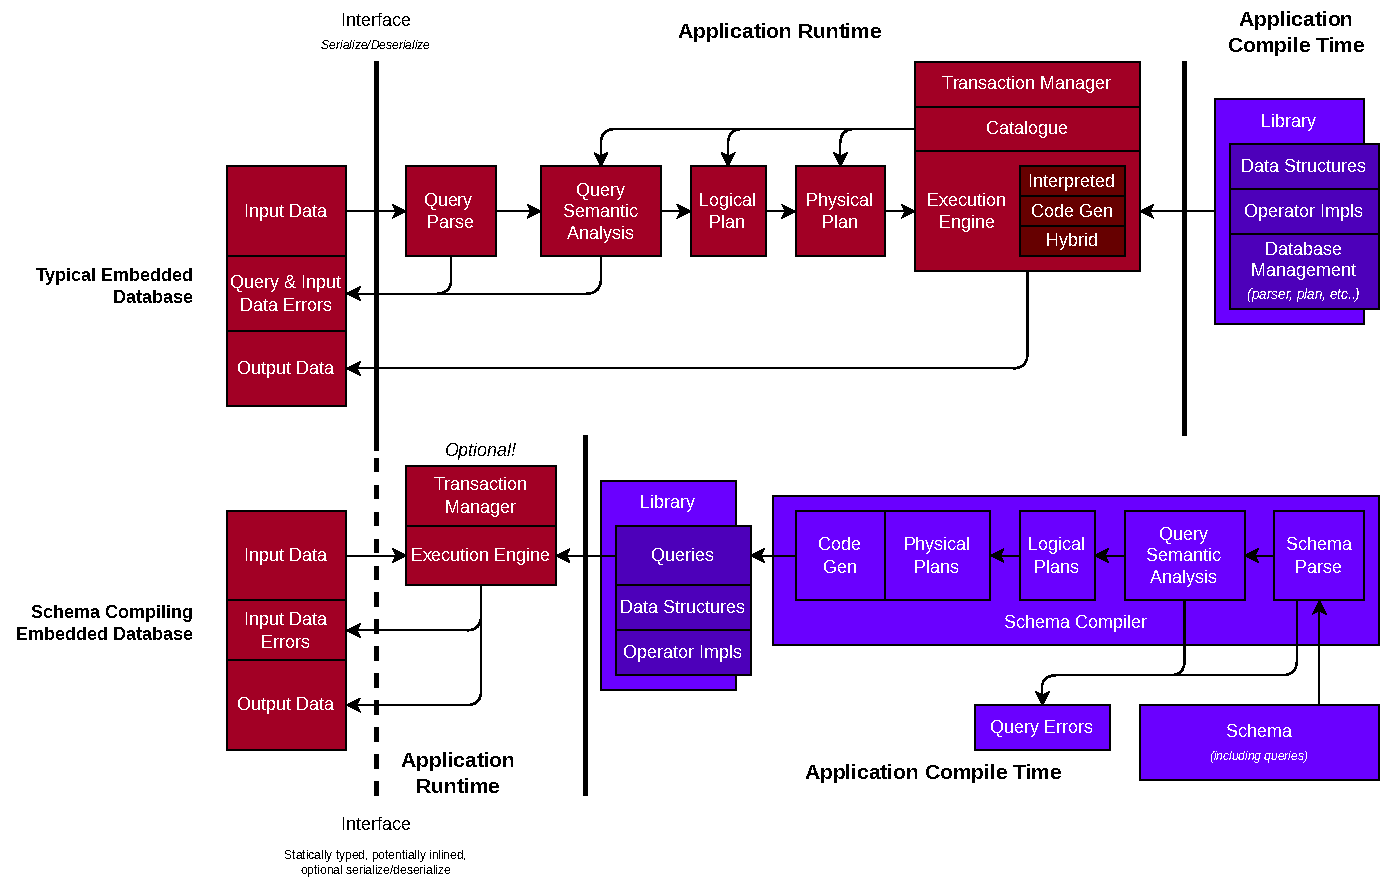
\includegraphics[width=\textwidth]{_diagrams/query_lifespan.pdf}
    \caption{A comparison of query lifespan for traditional and schema compililation based embedded databases}
    \label{fig:query-lifespan}
\end{figure*}

\subsection{Eliminating the Cost of Code Generation}
% In typical systems a careful balance between time spent on code generation (where high-level (whole compiler needed, but more checks & can be human readable for debugging) or 
% heavily optimised (optimiser takes time) code takes longer) and time on the query.
% - Discussed in Incremental Fusion 
% - Discussed in the hyper paper
% - One of the main disadvantages of HIQUE
% Significant effort in this area of reserach, we can blissfully do away with this complexity by moving 
% query compilation to application compile time, eliminating the entire runtime cost.

% Generating code in a high level language has additional benefits:
% - Easier to debug, including with standard tooling for the language (debuggers, profilers)
% - Easy to use with standard testing and benchmarking unitlities for the language
% - Can store types usable by the language (e.g. closures, custom user-defined data types)
% - Can rely on language semantics (e.g. move semantics, borrow checking for rust) and semantic analysis
% (e.g. type checking, rust guarentees on UB, memory safety) to validate code
% - Can be compiled alongside the application (e.g. inlining small queries, placing application logic
% in the database)

% More Human readable + more semantic checks + more optimisation = more costly, unless all done at compile time
In typical systems, achieving an optimal balance between the time spent on code generation and query
execution presents a significant challenge.

% list codegen databases
% Better because - inlining operator calls/volcano without call overhead + can use tight loops
Query complication is used by a growing number of systems, and can perform better than interpreted queries.

A more expensive query compiler can perform more semantic checks of generated
code (useful for correctness guarentees), compile higher level code (e.g. Rust or C++ rather than llvm, easier for development and debugging),
and perform more optimisation. The tradeoff between the performance advantage of codegen, and
the cost of compilation for a given query is lower, or even counterproductive for
small (typical OLTP) queries.

% 1. Just ignore for OLTP - does not matter for non-OLTP workloads (HIQUE)
% 2. Use a lower level representation (LLVM)
% 3. Reduce optimization
% 4. Cache query complications
% 5. Use interpreted queries for smaller query plans 
% 6. A form on JIT: Interpret the query while compiling, and switch 
There are several mitigations.
\begin{enumerate}
    \item Ignore the problem for non-OLTP workloads, and target the system for use in OLAP workloads where this is not a weakness. (\cite{HIQUE}) % HIQUE was only evalueted on large aggregations/joins, mentions cost of query compilation
    \item Generate a lower-level representation for query code to compile (e.g. LLVM IR or asm, instead of C++), at the cost of
          removing checking of queries (semantic analysis) and more difficult implementation. (\cite{HyperEfficientCompilation}, \cite{AdaptiveExecution}, \cite{PracticalCodegen}) % LLVM IR, hyper paper also has an asm backend and C++ backend to compare
    \item Reduce the level of optimisation performed, reduces the performance benefit of code generation.
    \item Cache query compilations to take advantage of repeat OLTP queries, some complexity is introduced to manage the cache. (\cite{MemSQL}) % memsql plan cache
    \item Hybrid execution of queries with an interpreter, before switching to the compiled version (a JIT-based system). (\cite{wagner2024incremental}, \cite{AdaptiveExecution}) % Both are JIT
\end{enumerate}
These mitigations are often complex to implement, and require a careful balance of trade-offs between performance for different 
kinds of workloads.

We choose to avoid tackling this hard problem. As we have the restriction that all parameterized queries are 
known, we can instead simply move query compilation from application runtime to application compile time.

This enables the maximal benefits of code generation (high level code, semantic analysis, expensive 
optimisations), with no runtime cost.

Furthermore as all queries and tables are generated at application compile time, the types of all data in all queries
and tables are known, meaning no explicit runtime type information or catalogue is required. This also allows arbitrary
types to used in the database (closures, custom user types, user data structures, smart pointers, etc.) and pure expressions 
(calling user defined functions) to be embedded into the database.

A significant difficulty with developing runtime codegen systems is tooling, for example requiring engine-integrated custom debuggers to be implemented.\cite{PracticalCodegen} 
Generating human readable code (compiled with the application) has auxiliary tooling benefits, it becomes easily usable with any tooling
available for the language, such as debuggers, profilers, testing, benchmarking and verification tools -
it's not a bespoke, complex runtime codegen system needing its own special tooling; it's \textit{just} (mostly human readable) code.  

\subsection{Compile Time Errors}
% Query errors (syntactic and semantic) can be reported at compile time and propagated to the IDE.
% Reduces time to write queries, no testing required.
% - Return types for queries only need to include errors only possible to detect at runtime, such as 
%   breaching unique constraints, or user assertions.

Query errors, both syntactic and semantic, can be detected and reported at compile time, and these errors
can be propagated to the Integrated Development Environment (IDE). This capability significantly reduces
the time required to check queries, without more compile-time complex debug database checking as in sqlx.

Furthermore, the return types for queries only need to include errors that can only be detected
at runtime. These include violations of unique constraints or user-defined assertions. By restricting
error handling to these specific cases, the overall complexity and overhead associated with query
execution are minimized, thereby enhancing both developer productivity and system reliability.

\begin{figure}[h]
    \begin{minted}[highlightlines=7,highlightcolor=red,linenos]{rust}
table people {
    name: String,
    friend: Option<String>,
} @ [ unique(name) as unique_names ]

query catalogue_error() {
    use not_people // no such table
        |> filter( name.len() < 10 ) 
        |> collect(users) 
        ~> return;
}
    \end{minted}
    \caption{A semantic error in IDE}
    \label{fig:query-error}
\end{figure}

\subsection{Data Structure Selection}
% Choosing Data Structure
% - Optimise choice of data structure for tables based on queries.
%
% For example determining which columns of a table are immutable, and which tables are append-only.
% - Immutable values, stored in a data structure that has pointer stability can return references 
%   qualified by the lifetime of the database, given values are not deleted or are reference counted.
% - Append only tables do not require a generation counter for row references

Choosing the optimal data structure for tables is a critical aspect of database performance optimization.
This choice is driven by the specific queries that will be executed.

For instance, identifying which columns of a table are immutable and which tables are append-only
allows for significant optimizations. Immutable values can be stored in a data structure with pointer
stability, enabling the return of references qualified by the lifetime of the database. This approach
ensures efficient access and manipulation of data.

Additionally, append-only tables benefit from not requiring a generation counter for row references,
simplifying their implementation and reducing overhead. By tailoring data structures to the characteristics
of the data and the nature of the queries, overall system efficiency and performance are greatly
enhanced.


Test\cite{wagner2024incremental}
\section{Implementation}

\subsection{Rust Procedural Macros}

\bibliographystyle{IEEEtran}
\bibliography{IEEEabrv,refs}

\end{document}
